\chapter{La symétrie axiale}
{https://sacado.xyz/qcm/parcours_show_course/0/117128}
{
\begin{CpsCol}
{\LARGE \textbf{\color{sacado_violet}{Les savoir faire ciblés}}}
\begin{itemize}[leftmargin=*]
\item Savoir déterminer si des points sont symétriques par rapport à une droite.
\item Savoir construire l'image d'un point, d'un segment, d'une droite, d'un cercle par une symétrie axiale.
\item Savoir construire l'image d'une figure par une symétrie axiale
\item Savoir compléter une figure par symétrie.
\item Savoir déterminer un axe de symétrie.
\item Savoir utiliser les axes de symétrie.
\item Savoir construire un axe de symétrie.
\end{itemize}
\end{CpsCol}


\begin{CCon}
{\LARGE \textbf{\color{sacado_violet}{Chapitres connexes spiralés}}}
\begin{itemize}[leftmargin=*]
\item Droites parallèles et perpendiculaires   
\end{itemize}
\end{CCon}

}




\begin{pageCours}

\section{La symétrie axiale}

\begin{DefT}{symétrie axiale}

\begin{minipage}{0.65\linewidth}
La \textbf{symétrie axiale}\index{symétrie axiale}  (par rapport à une droite) est une \textbf{transformation} du plan.

Elle transforme un point $A$ en un point $A'$ appelé image de $A$ par la transformation.
\end{minipage}
\hfill
\begin{minipage}{0.3\linewidth}
\begin{tikzpicture}[line cap=round,line join=round,>=triangle 45,x=1.0cm,y=1.0cm]
\clip(1.52,-1.4) rectangle (6.04,2.46);
\draw [color=ffqqqq](4.0,2.) node[anchor=north west] {$(d)$};
\draw [line width=1.pt,color=ffqqqq,domain=1.52:6.04] plot(\x,{(-7.24--2.46*\x)/1.3});
\begin{scriptsize}
\draw [color=ududff] (2.1,1.)-- ++(-2.5pt,0 pt) -- ++(5.0pt,0 pt) ++(-2.5pt,-2.5pt) -- ++(0 pt,5.0pt);
\draw[color=ududff] (2.24,1.37) node {$A$};
\draw [color=ududff] (4.24426991836313,-0.1331507698666945)-- ++(-2.5pt,0 pt) -- ++(5.0pt,0 pt) ++(-2.5pt,-2.5pt) -- ++(0 pt,5.0pt);
\draw[color=ududff] (4.44,0.23) node {$A'$};
\end{scriptsize}
\end{tikzpicture}
\end{minipage}
\end{DefT}
 

 

\section{Image d'un point par une symétrie axiale}

 

\begin{DefT}{Image d'un point} 



\begin{minipage}{0.6\linewidth}
L'\textbf{image} \index{Image d'un point|Symétrie axiale} d'un point $A$ par la symétrie axiale d'axe $(d)$ est le point $A'$ tel que :
\begin{itemize}
\item \textbf{Si} $A\in(d)$, \textbf{alors} $A$ et $A'$ sont confondus.
\item \textbf{Si} $A\notin(d)$, \textbf{alors} $(d)$ est la \textbf{médiatrice} du segment $[AA']$.
\end{itemize}
\end{minipage}
\begin{minipage}{0.4\linewidth}
\begin{tikzpicture}[line cap=round,line join=round,>=triangle 45,x=1.0cm,y=1.0cm]
\clip(6.202178380299732,-1.5) rectangle (12.096569942645493,2);
\draw[line width=1.pt,color=xdxdff,fill=xdxdff,fill opacity=0.10000000149011612] (9.074575961575169,0.724984335523733) -- (8.803735304729022,0.7749782202103872) -- (8.753741420042367,0.504137563364239) -- (9.024582076888516,0.4541436786775847) -- cycle; 
\draw [line width=1.pt,domain=6.202178380299732:12.096569942645493] plot(\x,{(--99.7788-11.16*\x)/-2.06});
\draw [line width=1.pt,dash pattern=on 1pt off 3pt] (6.8123907226571125,0.8624872440643847)-- (9.024582076888516,0.4541436786775847);
\draw [line width=1.pt] (7.932626805724729,0.7349207674017565) -- (7.904345993820897,0.5817101553402132);
\draw [line width=1.pt,dash pattern=on 1pt off 3pt] (9.024582076888516,0.4541436786775847)-- (11.236773431119914,0.04580011329078426);
\draw [line width=1.pt] (10.144818159956131,0.326577202014956) -- (10.116537348052296,0.17336658995341261);
\draw (9.3,1.5) node[anchor=north west] {$(d)$};
\draw [color=ududff] (6.8123907226571125,0.8624872440643847)-- ++(-2.5pt,-2.5pt) -- ++(5.0pt,5.0pt) ++(-5.0pt,0) -- ++(5.0pt,-5.0pt);
\draw[color=ududff] (6.903273411944382,1.1026772086093108) node {$A$};
\draw [color=ududff] (11.236773431119914,0.04580011329078426)-- ++(-2.5pt,-2.5pt) -- ++(5.0pt,5.0pt) ++(-5.0pt,0) -- ++(5.0pt,-5.0pt);
\draw[color=ududff] (11.369508428347338,0.28473300502388654) node {$A'$};
\draw [color=xdxdff] (8.786004044339178,-0.8383470219294955)-- ++(-2.5pt,0 pt) --
 ++(5.0pt,0 pt);% ++(-2.5pt,-2.5pt) -- ++(0 pt,5.0pt);
\draw[color=xdxdff] (8.5,-0.5981274051953017) node {$B$};
\draw[color=xdxdff] (9.2,-0.5981274051953017) node {$B'$};
\end{tikzpicture}
\end{minipage}
\end{DefT}
 

\begin{Mt}
\qr{•}{Déterminer la symétrie de 2 points par rapport à une droite}
\end{Mt}
\end{pageCours}



\begin{pageAD}
 
 
\Sf{Déterminer l'image d'un point par une symétrie axiale}


\begin{ExoCad}{Représenter.}{1234}{2}{0}{0}{0}{0}



\begin{minipage}{0.45\linewidth}

A l'aide de la figure ci-contre, trouve les points symétriques par rapport à la droite $(d)$.
 
\point{5}
 
\end{minipage}
\hfil
\begin{minipage}{0.58\linewidth}
\definecolor{ududff}{rgb}{0.30196078431372547,0.30196078431372547,1.}
\definecolor{ffqqqq}{rgb}{1.,0.,0.}
\definecolor{cqcqcq}{rgb}{0.7529411764705882,0.7529411764705882,0.7529411764705882}
\begin{tikzpicture}[line cap=round,line join=round,>=triangle 45,x=1.0cm,y=1.0cm]
\draw [color=cqcqcq,, xstep=1.0cm,ystep=1.0cm] (-3.44,1.2) grid (3.9,6.08);
\clip(-3.44,1.2) rectangle (3.9,6.08);
\draw [color=ffqqqq](0.06,6.18) node[anchor=north west] {$(d)$};
\draw [line width=1.pt,color=ffqqqq] (0.,1.2) -- (0.,6.08);
\begin{scriptsize}
\draw [color=ududff] (-2.,2.)-- ++(-2.5pt,0 pt) -- ++(5.0pt,0 pt) ++(-2.5pt,-2.5pt) -- ++(0 pt,5.0pt);
\draw[color=ududff] (-2.28,1.79) node {$A$};
\draw [color=ududff] (2.,2.)-- ++(-2.5pt,0 pt) -- ++(5.0pt,0 pt) ++(-2.5pt,-2.5pt) -- ++(0 pt,5.0pt);
\draw[color=ududff] (2.12,1.79) node {$B$};
\draw [color=ududff] (-1.,3.)-- ++(-2.5pt,0 pt) -- ++(5.0pt,0 pt) ++(-2.5pt,-2.5pt) -- ++(0 pt,5.0pt);
\draw[color=ududff] (-0.9,3.41) node {$C$};
\draw [color=ududff] (1.,3.)-- ++(-2.5pt,0 pt) -- ++(5.0pt,0 pt) ++(-2.5pt,-2.5pt) -- ++(0 pt,5.0pt);
\draw[color=ududff] (1.22,3.31) node {$D$};
\draw [color=ududff] (-2.,5.)-- ++(-2.5pt,0 pt) -- ++(5.0pt,0 pt) ++(-2.5pt,-2.5pt) -- ++(0 pt,5.0pt);
\draw[color=ududff] (-1.86,5.37) node {$E$};
\draw [color=ududff] (3.,3.)-- ++(-2.5pt,0 pt) -- ++(5.0pt,0 pt) ++(-2.5pt,-2.5pt) -- ++(0 pt,5.0pt);
\draw[color=ududff] (3.14,3.37) node {$F$};
\draw [color=ududff] (-2.,4.)-- ++(-2.5pt,0 pt) -- ++(5.0pt,0 pt) ++(-2.5pt,-2.5pt) -- ++(0 pt,5.0pt);
\draw[color=ududff] (-1.86,4.37) node {$G$};
\draw [color=ududff] (1.,4.)-- ++(-2.5pt,0 pt) -- ++(5.0pt,0 pt) ++(-2.5pt,-2.5pt) -- ++(0 pt,5.0pt);
\draw[color=ududff] (1.14,4.37) node {$H$};
\draw [color=ududff] (2.,4.)-- ++(-2.5pt,0 pt) -- ++(5.0pt,0 pt) ++(-2.5pt,-2.5pt) -- ++(0 pt,5.0pt);
\draw[color=ududff] (2.14,4.37) node {$I$};
\draw [color=ududff] (1.,5.)-- ++(-2.5pt,0 pt) -- ++(5.0pt,0 pt) ++(-2.5pt,-2.5pt) -- ++(0 pt,5.0pt);
\draw[color=ududff] (1.14,5.37) node {$J$};
\draw [color=ududff] (3.,4.)-- ++(-2.5pt,0 pt) -- ++(5.0pt,0 pt) ++(-2.5pt,-2.5pt) -- ++(0 pt,5.0pt);
\draw[color=ududff] (3.14,4.37) node {$K$};
\draw [color=ududff] (-3.,3.)-- ++(-2.5pt,0 pt) -- ++(5.0pt,0 pt) ++(-2.5pt,-2.5pt) -- ++(0 pt,5.0pt);
\draw[color=ududff] (-2.86,3.37) node {$L$};
\draw [color=ududff] (-1.,5.)-- ++(-2.5pt,0 pt) -- ++(5.0pt,0 pt) ++(-2.5pt,-2.5pt) -- ++(0 pt,5.0pt);
\draw[color=ududff] (-0.86,5.37) node {$M$};
\draw [color=ududff] (-2.,3.)-- ++(-2.5pt,0 pt) -- ++(5.0pt,0 pt) ++(-2.5pt,-2.5pt) -- ++(0 pt,5.0pt);
\draw[color=ududff] (-1.86,3.37) node {$N$};
\draw [color=ududff] (-1.,2.)-- ++(-2.5pt,0 pt) -- ++(5.0pt,0 pt) ++(-2.5pt,-2.5pt) -- ++(0 pt,5.0pt);
\draw[color=ududff] (-0.86,2.37) node {$O$};
\end{scriptsize}
\end{tikzpicture}
\end{minipage}

\end{ExoCad}
\begin{ExoCad}{Représenter.}{1234}{2}{0}{0}{0}{0}


\begin{minipage}{0.48\linewidth}
On donne 4 points, A, B, C et D.

Quel point semble-t-il être le point symétrique de A par la symétrie d'axe $(d)$ ? 
\vspace{0.4cm}
$\ldots\ldots$
\end{minipage}
\hfill
\begin{minipage}{0.48\linewidth}
\definecolor{ffqqqq}{rgb}{1.,0.,0.}
\definecolor{ududff}{rgb}{0.30196078431372547,0.30196078431372547,1.}
\begin{tikzpicture}[line cap=round,line join=round,>=triangle 45,x=1.0cm,y=1.0cm]
\clip(-2.54,-0.26) rectangle (2.7,2.9);
\draw [line width=1.pt,color=ffqqqq,domain=-2.54:2.7] plot(\x,{(--2.676--0.68*\x)/1.16});
\draw [color=ffqqqq](1.04,2.74) node[anchor=north west] {$(d)$};
\begin{scriptsize}
\draw [color=ududff] (-2.16,1.82)-- ++(-2.5pt,0 pt) -- ++(5.0pt,0 pt) ++(-2.5pt,-2.5pt) -- ++(0 pt,5.0pt);
\draw[color=ududff] (-2.02,2.19) node {$A$};
\draw [color=ududff] (-1.48,0.66)-- ++(-2.5pt,0 pt) -- ++(5.0pt,0 pt) ++(-2.5pt,-2.5pt) -- ++(0 pt,5.0pt);
\draw[color=ududff] (-1.18,0.63) node {$B$};
\draw [color=ududff] (-1.28,1.88)-- ++(-2.5pt,0 pt) -- ++(5.0pt,0 pt) ++(-2.5pt,-2.5pt) -- ++(0 pt,5.0pt);
\draw[color=ududff] (-1.14,2.25) node {$D$};
\draw [color=ududff] (0.36,1.88)-- ++(-2.5pt,0 pt) -- ++(5.0pt,0 pt) ++(-2.5pt,-2.5pt) -- ++(0 pt,5.0pt);
\draw[color=ududff] (0.5,2.25) node {$E$};
\end{scriptsize}
\end{tikzpicture}
\end{minipage}

\end{ExoCad}
\begin{ExoCad}{Représenter.}{1234}{2}{0}{0}{0}{0}

 
\begin{minipage}{0.58\linewidth}

A l'aide de la figure ci-dessous, nomme le point symétrique de chaque point par rapport à la droite $(d)$.
 
\begin{enumerate}
\item Le symétrique du point $A$ par rapport à la droite $(d)$ est le point $\ldots\ldots$.\vspace{0.2cm}
\item Le symétrique du point $N$ par rapport à la droite $(d)$ est le point $\ldots\ldots$.\vspace{0.2cm}
\item Le symétrique du point $M$ par rapport à la droite $(d)$ est le point $\ldots\ldots$.
\end{enumerate}

\end{minipage}
\hfill
\begin{minipage}{0.38\linewidth}

\definecolor{ffqqqq}{rgb}{1.,0.,0.}
\definecolor{ududff}{rgb}{0.30196078431372547,0.30196078431372547,1.}
\begin{tikzpicture}[line cap=round,line join=round,>=triangle 45,x=1.0cm,y=1.0cm]
\clip(-2.82,0.34) rectangle (2.94,5.58);
\draw[line width=1.pt] (0.17981245261632933,2.4538239307035883) -- (0.38144325484736674,2.827113388888076) -- (0.008153796662878854,3.0287441911191135) -- (-0.1934770055681585,2.6554547329346256) -- cycle; 
\draw[line width=1.pt] (-0.4767105418155122,1.2383691977689626) -- (-0.27507973958447496,1.6116586559534505) -- (-0.6483691977689628,1.8132894581844878) -- (-0.85,1.44) -- cycle; 
\draw[line width=1.pt] (0.943710988396903,3.868068517216271) -- (1.1453417906279402,4.241357975400759) -- (0.7720523324434524,4.442988777631797) -- (0.5704215302124152,4.069699319447309) -- cycle; 
\draw [line width=1.pt,color=ffqqqq,domain=-2.82:2.94] plot(\x,{(--4.4602--2.74*\x)/1.48});
\draw [color=ffqqqq](1.22,5.62) node[anchor=north west] {$(d)$};
\draw [line width=1.pt] (-2.22,2.18)-- (-0.85,1.44);
\draw [line width=1.pt] (-1.4779701969785402,1.9155822028910816) -- (-1.59202980302146,1.704417797108919);
\draw [line width=1.pt] (-0.85,1.44)-- (0.52,0.7);
\draw [line width=1.pt] (-0.10797019697854016,1.1755822028910818) -- (-0.22202980302145997,0.9644177971089193);
\draw [line width=1.pt] (-0.29915693957516964,4.5393986388946175)-- (1.44,3.6);
\draw [line width=1.pt] (1.333045988863683,1.830909465869251)-- (-1.72,3.48);
\draw [line width=1.pt] (-1.72,3.48)-- (-0.1934770055681585,2.6554547329346256);
\draw [line width=1.pt] (-0.9876938688385198,3.220834405209611) -- (-1.1017534748814397,3.0096699994274485);
\draw [line width=1.pt] (-0.8997086997626187,3.1733095693583944) -- (-1.0137683058055384,2.9621451635762317);
\draw [line width=1.pt] (-0.8117235306867175,3.1257847335071776) -- (-0.9257831367296374,2.914620327725015);
\draw [line width=1.pt] (-0.1934770055681585,2.6554547329346256)-- (1.333045988863683,1.830909465869251);
\draw [line width=1.pt] (0.5388291255933213,2.3962891381442364) -- (0.4247695195504015,2.1851247323620737);
\draw [line width=1.pt] (0.6268142946692219,2.3487643022930196) -- (0.5127546886263021,2.137599896510857);
\draw [line width=1.pt] (0.7147994637451225,2.3012394664418023) -- (0.6007398577022027,2.09007506065964);
\draw [line width=1.pt] (1.44,3.6)-- (0.5704215302124152,4.069699319447309);
\draw [line width=1.pt] (0.9921735466226986,3.705505038906964) -- (1.1062331526656184,3.9166694446891266);
\draw [line width=1.pt] (0.904188377546798,3.7530298747581807) -- (1.0182479835897178,3.9641942805403434);
\draw [line width=1.pt] (0.5704215302124152,4.069699319447309)-- (-0.29915693957516964,4.5393986388946175);
\draw [line width=1.pt] (0.12259507683511292,4.175204358354272) -- (0.23665468287803273,4.386368764136435);
\draw [line width=1.pt] (0.034609907759212334,4.222729194205489) -- (0.14866951380213214,4.433893599987652);
\begin{scriptsize}
\draw [color=ududff] (-2.22,2.18)-- ++(-2.5pt,0 pt) -- ++(5.0pt,0 pt) ++(-2.5pt,-2.5pt) -- ++(0 pt,5.0pt);
\draw[color=ududff] (-2.08,2.55) node {$A$};
\draw [color=ududff] (0.52,0.7)-- ++(-2.5pt,0 pt) -- ++(5.0pt,0 pt) ++(-2.5pt,-2.5pt) -- ++(0 pt,5.0pt);
\draw[color=ududff] (0.82,0.67) node {$B$};
\draw [color=ududff] (-1.72,3.48)-- ++(-2.5pt,0 pt) -- ++(5.0pt,0 pt) ++(-2.5pt,-2.5pt) -- ++(0 pt,5.0pt);
\draw[color=ududff] (-1.58,3.85) node {$D$};
\draw [color=ududff] (1.44,3.6)-- ++(-2.5pt,0 pt) -- ++(5.0pt,0 pt) ++(-2.5pt,-2.5pt) -- ++(0 pt,5.0pt);
\draw[color=ududff] (1.58,3.97) node {$E$};
\draw [color=ududff] (-0.29915693957516964,4.5393986388946175)-- ++(-2.5pt,0 pt) -- ++(5.0pt,0 pt) ++(-2.5pt,-2.5pt) -- ++(0 pt,5.0pt);
\draw[color=ududff] (-0.16,4.91) node {$N$};
\draw [color=ududff] (1.333045988863683,1.830909465869251)-- ++(-2.5pt,0 pt) -- ++(5.0pt,0 pt) ++(-2.5pt,-2.5pt) -- ++(0 pt,5.0pt);
\draw[color=ududff] (1.48,2.21) node {$M$};
\end{scriptsize}
\end{tikzpicture}
\end{minipage}

\end{ExoCad}

\end{pageAD}

\begin{pageCours}

\section{Construire le symétrique d'un point, d'une figure}

\begin{Mt}
Pour construire le symétrique d'un point par rapport à une droite, on peut utiliser le quadrillage du papier ou une équerre ou un compas et une règle.
\end{Mt}

\section{Propriétés de la symétrie axiale}

 
\begin{Pp}
La symétrie axiale conserve :
\begin{itemize}
\item L'\textbf{alignement} (les symétriques de trois points alignés sont aussi alignés.)
\item Les \textbf{distances} (la distance entre deux points est la même que celle entre leur symétrique).
\item Les \textbf{mesures d'angles} (le symétrique d'un angle est un angle de même mesure).
\end{itemize}
\end{Pp} 
 
\begin{Cq}
$A'$ est le symétrique de $A$, $B'$ est le symétrique de $B$ ET $C'$ est le symétrique de $C$ par une symétrie axiale d'axe $(d)$. 
\begin{itemize}
\item L'image d'un segment est un segment de même longueur.
\item L'image d'une droite est une droite.
\item L'image d'un cercle est un cercle de même rayon.
\end{itemize}

\begin{minipage}[c]{.3\linewidth}
\begin{center}
\textbf{Alignement}

\vspace{.2cm}
\begin{tikzpicture}[line cap=round,line join=round,>=triangle 45,x=0.6cm,y=0.6cm]
\clip(5.773731416516891,-2.5391219835448404) rectangle (11.966737529377966,3.199470682879883);
\draw [line width=1.pt,domain=5.773731416516891:11.966737529377966,color=sacado_blue] plot(\x,{(--99.7788-11.16*\x)/-2.06});
\draw [color=sacado_blue](9.455720573215971,2.978755580325086) node[anchor=north west] {$(d)$};
\draw [line width=1.pt,dash pattern=on 1pt off 3pt,domain=5.773731416516891:11.966737529377966] plot(\x,{(--10.076771316934485-1.4281565459428047*\x)/-0.5972291010306279});
\draw [line width=1.pt,dash pattern=on 1pt off 3pt,domain=5.773731416516891:11.966737529377966] plot(\x,{(--16.525680188028545-1.5472586604476053*\x)/0.04800371347110721});
\draw [color=black] (7.318737134400471,0.628788900182835)-- ++(-2.5pt,-2.5pt) -- ++(5.0pt,5.0pt) ++(-5.0pt,0) -- ++(5.0pt,-5.0pt);
\draw[color=black] (7.80961982368774,0.8689788647277612) node {$B$};
\draw [color=black] (10.680362265288089,0.008273867062001505)-- ++(-2.5pt,-2.5pt) -- ++(5.0pt,5.0pt) ++(-5.0pt,0) -- ++(5.0pt,-5.0pt);
\draw[color=black] (11.21122905129697,0.24578328104362823) node {$B'$};
\draw [color=black] (6.721508033369843,-0.7993676457599697)-- ++(-2.5pt,-2.5pt) -- ++(5.0pt,5.0pt) ++(-5.0pt,0) -- ++(5.0pt,-5.0pt);
\draw[color=black] (7.2123907226571125,-0.5591776812150434) node {$C$};
\draw [color=black] (7.860763497564994,1.9249388990545202)-- ++(-2.5pt,-2.5pt) -- ++(5.0pt,5.0pt) ++(-5.0pt,0) -- ++(5.0pt,-5.0pt);
\draw[color=black] (8.254915959411357,2.167302997403038) node {$A$};
\draw [color=black] (10.728365978759197,-1.5389847933856038)-- ++(-2.5pt,-2.5pt) -- ++(5.0pt,5.0pt) ++(-5.0pt,0) -- ++(5.0pt,-5.0pt);
\draw[color=black] (11.26316201660398,-1.2992224368399512) node {$C'$};
\draw [color=black] (10.636795603539298,1.4125172020735999)-- ++(-2.5pt,-2.5pt) -- ++(5.0pt,5.0pt) ++(-5.0pt,0) -- ++(5.0pt,-5.0pt);
\draw[color=black] (11.17227932731671,1.6479733443329272) node {$A'$};
\end{tikzpicture}
\end{center}
\end{minipage}
\hfill % espace horizontal
\vline % ligne verticale
\hfill % espace horizontal
\begin{minipage}[c]{.3\linewidth}
\begin{center}
\textbf{Distance}

\vspace{.2cm}
\begin{tikzpicture}[line cap=round,line join=round,>=triangle 45,x=0.6cm,y=0.6cm]
\clip(5.773731416516891,-2.5391219835448404) rectangle (11.966737529377966,3.199470682879883);
\draw [line width=1.pt,domain=0.5025354378552631:21.327654525966718,color=sacado_violet] plot(\x,{(--99.7788-11.16*\x)/-2.06});
\draw [color=sacado_violet](9.655720573215971,2.978755580325086) node[anchor=north west] {$(d)$};
\draw [line width=1.pt] (7.318737134400471,0.628788900182835)-- (7.8121003048170765,-0.8772670937204862);
\draw [line width=1.pt] (10.680362265288089,0.008273867062001505)-- (9.681832684528693,-1.2223969057461075);
\draw [color=ududff] (7.318737134400471,0.628788900182835)-- ++(-2.5pt,-2.5pt) -- ++(5.0pt,5.0pt) ++(-5.0pt,0) -- ++(5.0pt,-5.0pt);
\draw[color=ududff] (7.70961982368774,0.8689788647277612) node {$A$};
\draw [color=ududff] (10.680362265288089,0.008273867062001505)-- ++(-2.5pt,-2.5pt) -- ++(5.0pt,5.0pt) ++(-5.0pt,0) -- ++(5.0pt,-5.0pt);
\draw[color=ududff] (11.21122905129697,0.24578328104362823) node {$A'$};
\draw [color=ududff] (7.8121003048170765,-0.8772670937204862)-- ++(-2.5pt,-2.5pt) -- ++(5.0pt,5.0pt) ++(-5.0pt,0) -- ++(5.0pt,-5.0pt);
\draw[color=ududff] (8.202982994104346,-0.63707712917556) node {$B$};
\draw [color=ududff] (9.681832684528693,-1.2223969057461075)-- ++(-2.5pt,-2.5pt) -- ++(5.0pt,5.0pt) ++(-5.0pt,0) -- ++(5.0pt,-5.0pt);
\draw[color=ududff] (9.311519469137005,-0.9876246449978848) node {$B'$};
\end{tikzpicture}

$AB=A'B'$
\end{center}
\end{minipage}
\hfill % espace horizontal
\vline % ligne verticale
\hfill % espace horizontal
\begin{minipage}[c]{.3\linewidth}
\begin{center}
\textbf{Angles}

\vspace{.2cm}
\begin{tikzpicture}[line cap=round,line join=round,>=triangle 45,x=0.7cm,y=0.7cm]
\clip(5.773731416516891,-2.5391219835448404) rectangle (11.966737529377966,3.199470682879883);
\draw [shift={(7.8121003048170765,-0.8772670937204862)},line width=1.pt,color=qqwuqq,fill=qqwuqq,fill opacity=0.10000000149011612] (0,0) -- (108.13808215559735:0.38949723980258333) arc (108.13808215559735:170.99824487743874:0.38949723980258333) -- cycle;
\draw [shift={(9.681832684528693,-1.2223969057461075)},line width=1.pt,color=qqwuqq,fill=qqwuqq,fill opacity=0.10000000149011612] (0,0) -- (-11.915007777236106:0.38949723980258333) arc (-11.915007777236106:50.94515494460531:0.38949723980258333) -- cycle;
\draw [line width=1.pt,domain=0.5025354378552631:21.327654525966718,color=red] plot(\x,{(--99.7788-11.16*\x)/-2.06});
\draw [color=red](9.655720573215971,2.978755580325086) node[anchor=north west] {$(d)$};
\draw [line width=1.pt] (7.318737134400471,0.628788900182835)-- (7.8121003048170765,-0.8772670937204862);
\draw [line width=1.pt] (10.680362265288089,0.008273867062001505)-- (9.681832684528693,-1.2223969057461075);
\draw [line width=1.pt] (7.8121003048170765,-0.8772670937204862)-- (6.500792930815046,-0.669535232492442);
\draw [line width=1.pt] (9.681832684528693,-1.2223969057461075)-- (10.980887609172752,-1.49650611398141);
\draw [color=black] (7.318737134400471,0.628788900182835)-- ++(-2.5pt,-2.5pt) -- ++(5.0pt,5.0pt) ++(-5.0pt,0) -- ++(5.0pt,-5.0pt);
\draw[color=black] (7.60961982368774,1.) node {$A$};
\draw [color=black] (10.680362265288089,0.008273867062001505)-- ++(-2.5pt,-2.5pt) -- ++(5.0pt,5.0pt) ++(-5.0pt,0) -- ++(5.0pt,-5.0pt);
\draw[color=black] (11.01122905129697,0.24578328104362823) node {$A'$};
\draw [color=black] (7.8121003048170765,-0.8772670937204862)-- ++(-2.5pt,-2.5pt) -- ++(5.0pt,5.0pt) ++(-5.0pt,0) -- ++(5.0pt,-5.0pt);
\draw[color=black] (8.02982994104346,-0.63707712917556) node {$B$};
\draw [color=black] (9.681832684528693,-1.2223969057461075)-- ++(-2.5pt,-2.5pt) -- ++(5.0pt,5.0pt) ++(-5.0pt,0) -- ++(5.0pt,-5.0pt);
\draw[color=black] (9.411519469137005,-0.9876246449978848) node {$B'$};
\draw [color=black] (6.500792930815046,-0.669535232492442)-- ++(-2.5pt,-2.5pt) -- ++(5.0pt,5.0pt) ++(-5.0pt,0) -- ++(5.0pt,-5.0pt);
\draw[color=black] (6.291675620102316,-0.3293452679475157) node {$C$};
\draw [color=black] (10.980887609172752,-1.49650611398141)-- ++(-2.5pt,-2.5pt) -- ++(5.0pt,5.0pt) ++(-5.0pt,0) -- ++(5.0pt,-5.0pt);
\draw[color=black] (11.409843601812281,-1.260272712859693) node {$C'$};
\end{tikzpicture}

$\widehat{ABC}=\widehat{A'B'C'}$
\end{center}
\end{minipage}


\end{Cq} 

 
 
\end{pageCours}

\begin{pageAD}

\Sf{Construire l'image d'un point par une symétrie axiale}


\begin{ExoCad}{Représenter.}{1234}{2}{0}{0}{0}{0}

Construis la figure symétrique par rapport à la droite $d$.

\definecolor{zzttqq}{rgb}{0.6,0.2,0.}
\definecolor{ffqqqq}{rgb}{1.,0.,0.}
\definecolor{cqcqcq}{rgb}{0.7529411764705882,0.7529411764705882,0.7529411764705882}
\begin{tikzpicture}[line cap=round,line join=round,>=triangle 45,x=1.0cm,y=1.0cm]
\draw [color=cqcqcq,, xstep=1.0cm,ystep=1.0cm] (-1.52,-1.7) grid (13.48,4.7);
\clip(-1.52,-1.7) rectangle (13.48,4.7);
\draw [line width=1.pt,color=ffqqqq] (-1.,4.)-- (3.,4.);
\draw [line width=1.pt,color=ffqqqq] (3.,4.)-- (3.,3.);
\draw [line width=1.pt,color=ffqqqq] (3.,3.)-- (0.,3.);
\draw [line width=1.pt,color=ffqqqq] (0.,3.)-- (0.,0.);
\draw [line width=1.pt,color=ffqqqq] (0.,0.)-- (4.,0.);
\draw [line width=1.pt,color=ffqqqq] (4.,0.)-- (4.,-1.);
\draw [line width=1.pt,color=ffqqqq] (4.,-1.)-- (-1.,-1.);
\draw [line width=1.pt,color=ffqqqq] (-1.,-1.)-- (-1.,4.);
\draw [line width=1.pt] (5.,-1.7) -- (5.,4.7);
\begin{scriptsize}
\draw [color=ffqqqq] (-1.,4.)-- ++(-2.5pt,0 pt) -- ++(5.0pt,0 pt) ++(-2.5pt,-2.5pt) -- ++(0 pt,5.0pt);
\draw[color=ffqqqq] (-0.86,4.37) node {$A$};
\draw [color=ffqqqq] (3.,4.)-- ++(-2.5pt,0 pt) -- ++(5.0pt,0 pt) ++(-2.5pt,-2.5pt) -- ++(0 pt,5.0pt);
\draw[color=ffqqqq] (3.14,4.37) node {$B$};
\draw[color=ffqqqq] (5.14,4.37) node {$(d)$};
\draw [color=ffqqqq] (3.,3.)-- ++(-2.5pt,0 pt) -- ++(5.0pt,0 pt) ++(-2.5pt,-2.5pt) -- ++(0 pt,5.0pt);
\draw[color=ffqqqq] (3.14,3.37) node {$C$};
\draw [color=ffqqqq] (0.,3.)-- ++(-2.5pt,0 pt) -- ++(5.0pt,0 pt) ++(-2.5pt,-2.5pt) -- ++(0 pt,5.0pt);
\draw[color=ffqqqq] (0.14,3.37) node {$D$};
\draw [color=ffqqqq] (0.,0.)-- ++(-2.5pt,0 pt) -- ++(5.0pt,0 pt) ++(-2.5pt,-2.5pt) -- ++(0 pt,5.0pt);
\draw[color=ffqqqq] (0.14,0.37) node {$E$};
\draw [color=ffqqqq] (4.,0.)-- ++(-2.5pt,0 pt) -- ++(5.0pt,0 pt) ++(-2.5pt,-2.5pt) -- ++(0 pt,5.0pt);
\draw[color=ffqqqq] (4.14,0.37) node {$F$};
\draw [color=ffqqqq] (4.,-1.)-- ++(-2.5pt,0 pt) -- ++(5.0pt,0 pt) ++(-2.5pt,-2.5pt) -- ++(0 pt,5.0pt);
\draw[color=ffqqqq] (4.14,-0.63) node {$G$};
\draw [color=ffqqqq] (-1.,-1.)-- ++(-2.5pt,0 pt) -- ++(5.0pt,0 pt) ++(-2.5pt,-2.5pt) -- ++(0 pt,5.0pt);
\draw[color=ffqqqq] (-0.86,-0.63) node {$H$};
\draw[color=black] (5.2,4.99) node {$d$};
\end{scriptsize}
\end{tikzpicture}
 
\end{ExoCad}
\begin{ExoCad}{Représenter.}{1234}{2}{0}{0}{0}{0}



\begin{minipage}{0.48\linewidth}

Construis l'image des points $A$, $B$ et $C$ dans la symétrie axiale d'axe $(d)$.

\begin{center}
\definecolor{ududff}{rgb}{0.30196078431372547,0.30196078431372547,1.}
\definecolor{ffqqqq}{rgb}{1.,0.,0.}
\begin{tikzpicture}[line cap=round,line join=round,>=triangle 45,x=1.0cm,y=1.0cm]
\clip(-3.14,1.02) rectangle (2.06,5.68);
\draw [color=ffqqqq](-0.96,5.8) node[anchor=north west] {$(d)$};
\draw [line width=2.pt,color=ffqqqq] (-1.,1.02) -- (-1.,5.68);
\begin{scriptsize}
\draw [color=ududff] (-1.78,4.46)-- ++(-2.5pt,0 pt) -- ++(5.0pt,0 pt) ++(-2.5pt,-2.5pt) -- ++(0 pt,5.0pt);
\draw[color=ududff] (-1.64,4.83) node {$A$};
\draw [color=ududff] (0.,3.)-- ++(-2.5pt,0 pt) -- ++(5.0pt,0 pt) ++(-2.5pt,-2.5pt) -- ++(0 pt,5.0pt);
\draw[color=ududff] (0.14,3.37) node {$B$};
\draw [color=ududff] (-2.42,1.72)-- ++(-2.5pt,0 pt) -- ++(5.0pt,0 pt) ++(-2.5pt,-2.5pt) -- ++(0 pt,5.0pt);
\draw[color=ududff] (-2.28,2.09) node {$C$};
\end{scriptsize}
\end{tikzpicture}
\end{center}

\end{minipage}
\hfill\vrule\hfill
\begin{minipage}{0.48\linewidth}

Construis l'image des points $D$, $E$ et $F$ dans la symétrie axiale d'axe $(d)$.

\begin{center}
\begin{tikzpicture}[line cap=round,line join=round,>=triangle 45,x=1.0cm,y=1.0cm]
\clip(-3.02,0.94) rectangle (1.3,5.64);
\draw [color=ffqqqq](-0.34,5.62) node[anchor=north west] {$(d)$};
\draw [line width=1.pt,color=ffqqqq,domain=-3.02:1.3] plot(\x,{(--10.68--5.9*\x)/1.78});
\begin{scriptsize}
\draw [color=ududff] (-1.78,4.46)-- ++(-2.5pt,0 pt) -- ++(5.0pt,0 pt) ++(-2.5pt,-2.5pt) -- ++(0 pt,5.0pt);
\draw[color=ududff] (-1.64,4.83) node {$F$};
\draw [color=ududff] (0.26,2.36)-- ++(-2.5pt,0 pt) -- ++(5.0pt,0 pt) ++(-2.5pt,-2.5pt) -- ++(0 pt,5.0pt);
\draw[color=ududff] (0.4,2.73) node {$E$};
\draw [color=ududff] (-2.42,1.72)-- ++(-2.5pt,0 pt) -- ++(5.0pt,0 pt) ++(-2.5pt,-2.5pt) -- ++(0 pt,5.0pt);
\draw[color=ududff] (-2.28,2.09) node {$D$};
\end{scriptsize}
\end{tikzpicture}
\end{center}
\end{minipage}


\end{ExoCad}
\begin{ExoCad}{Représenter.}{1234}{2}{0}{0}{0}{0}


\begin{minipage}{0.48\linewidth}
\begin{enumerate}
\item Trace la médiatrice du segment $[AB]$.
\item Code la figure.
\item Construis le symétrique du point $C$, noté $C'$. Compare $AC$ et $BC'$.
\end{enumerate}
\end{minipage}
 \hfill\vrule\hfill
\begin{minipage}{0.48\linewidth}
\begin{tikzpicture}[line cap=round,line join=round,>=triangle 45,x=1.0cm,y=1.0cm]
\clip(-4.92,0.9) rectangle (1.08,3.2);
\begin{scriptsize}
\draw [color=ududff] (-4.,2.)-- ++(-2.5pt,0 pt) -- ++(5.0pt,0 pt) ++(-2.5pt,-2.5pt) -- ++(0 pt,5.0pt);
\draw[color=ududff] (-4.3,2.41) node {$A$};
\draw [color=ududff] (0.,2.5)-- ++(-2.5pt,0 pt) -- ++(5.0pt,0 pt) ++(-2.5pt,-2.5pt) -- ++(0 pt,5.0pt);
\draw[color=ududff] (0.14,2.37) node {$B$};
\draw [color=ududff] (-3.,1.)-- ++(-2.5pt,0 pt) -- ++(5.0pt,0 pt) ++(-2.5pt,-2.5pt) -- ++(0 pt,5.0pt);
\draw[color=ududff] (-3.26,1.37) node {$C$};
\end{scriptsize}
\end{tikzpicture}
\end{minipage}

\end{ExoCad}
 

\end{pageAD}

\begin{pageCours}

\section{Axes de symétrie d'une figure}

\begin{DefT}{axe de symétrie}
Une droite $(d)$ est un \textbf{axe de symétrie}\index{axe de symétrie} d'une figure, si les deux parties de la figure se \textbf{superposent} par un pliage le long de la droite $(d)$.
\end{DefT}

\begin{Cq}
\begin{itemize}[leftmargin=*]
\item Par une symétrie axiale, l'image d'un polygone est un polygone de même forme et de mêmes dimensions.
\item L'axe de symétrie d'une figure est la \textbf{médiatrice}\index{Médiatrice} d'un point et de son symétrique.
\end{itemize}
\end{Cq}


\begin{PpT}{Axes de symétrie des figures usuelles}
\begin{center}
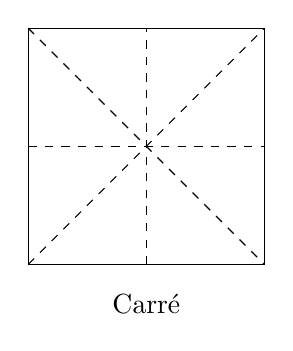
\begin{tikzpicture}[scale=0.5]
% Carré
\draw (0,0) rectangle (6,6);
\draw[dashed] (0,3) -- (6,3); % Axe de symétrie horizontal
\draw[dashed] (3,0) -- (3,6); % Axe de symétrie vertical
\draw[dashed] (0,6) -- (6,0); % Axe de symétrie diagonale haut-bas
\draw[dashed] (0,0) -- (6,6); % Axe de symétrie diagonale bas-haut
\node at (3,-1) {Carré};
\end{tikzpicture}
\hspace{1cm}
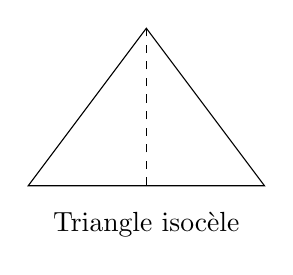
\begin{tikzpicture}[scale=0.5]
% Triangle isocèle
\draw (0,0) -- (6,0) -- (3,4) -- cycle;
\draw[dashed] (3,0) -- (3,4); % Axe de symétrie vertical
\node at (3,-1) {Triangle isocèle};
\end{tikzpicture}
\hspace{1cm}
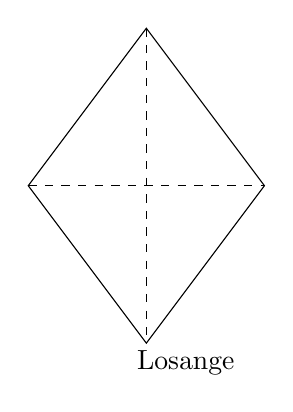
\begin{tikzpicture}[scale=0.5]
% Losange
\draw (0,0) -- (3,4) -- (6,0) -- (3,-4) -- cycle;
\draw[dashed] (3,4) -- (3,-4); % Axe de symétrie vertical
\draw[dashed] (0,0) -- (6,0); % Axe de symétrie horizontal
\node at (4,-4.5) {Losange};
\end{tikzpicture}

\vspace{1cm}

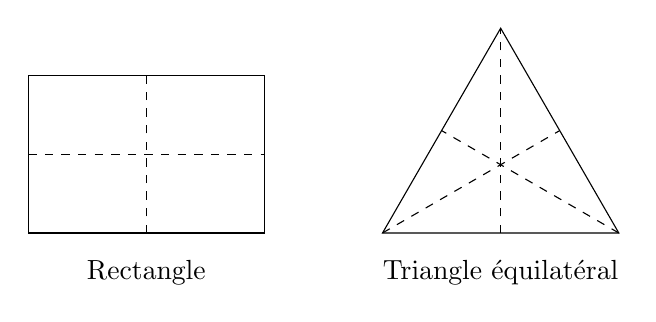
\begin{tikzpicture}[scale=0.5]
% Rectangle
\draw (-9,0) rectangle (-3,4);
\draw[dashed] (-6,0) -- (-6,4); % Axe de symétrie vertical
\draw[dashed] (-9,2) -- (-3,2); % Axe de symétrie horizontal
\node at (-6,-1) {Rectangle};

% Triangle équilatéral
\draw (0,0) -- (6,0) -- (3,5.2) -- cycle;
\draw[dashed] (3,0) -- (3,5.2); % Axe de symétrie vertical
\draw[dashed] (6,0) -- (1.5,2.6); % Axe de symétrie sommet droit
\draw[dashed] (0,0) -- (4.5,2.6); % Axe de symétrie sommet gauche
\node at (3,-1) {Triangle équilatéral};
\end{tikzpicture}
\hspace{1cm}
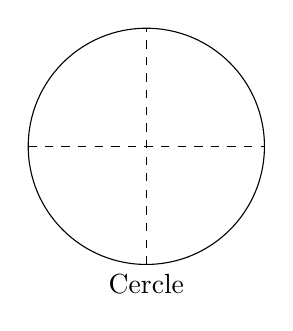
\begin{tikzpicture}[scale=0.5]
% Cercle
\draw (0,0) circle (3);
\draw[dashed] (-3,0) -- (3,0); % Axe de symétrie horizontal
\draw[dashed] (0,-3) -- (0,3); % Axe de symétrie vertical
\node at (0,-3.5) {Cercle};
\end{tikzpicture}
\end{center}
\end{PpT}

\end{pageCours}


\begin{pageAD} 
 

\Sf{Construire l'axe de symétrie d'une figure donnée}
 
  
\begin{ExoCad}{Représenter.}{1234}{2}{0}{0}{0}{0}


\definecolor{ududff}{rgb}{0.30196078431372547,0.30196078431372547,1.}
\definecolor{cqcqcq}{rgb}{0.7529411764705882,0.7529411764705882,0.7529411764705882}

\begin{minipage}{0.48\linewidth}
\begin{tikzpicture}[line cap=round,line join=round,>=triangle 45,x=1.0cm,y=1.0cm]
\draw [color=cqcqcq,, xstep=0.5cm,ystep=0.5cm] (-4.92,0.9) grid (1.08,3.2);
\clip(-4.92,0.9) rectangle (1.08,3.2);
\begin{scriptsize}
\draw [color=ududff] (-4.,2.)-- ++(-2.5pt,0 pt) -- ++(5.0pt,0 pt) ++(-2.5pt,-2.5pt) -- ++(0 pt,5.0pt);
\draw[color=ududff] (-4.3,2.41) node {$A$};
\draw [color=ududff] (0.,2.)-- ++(-2.5pt,0 pt) -- ++(5.0pt,0 pt) ++(-2.5pt,-2.5pt) -- ++(0 pt,5.0pt);
\draw[color=ududff] (0.14,2.37) node {$B$};
\end{scriptsize}
\end{tikzpicture}

\begin{enumerate}[leftmargin=*]
\item Dessine la médiatrice du segment $[AB]$.
\item Code la figure
\end{enumerate}
 \end{minipage}
\hfill\vrule\hfill
 \begin{minipage}{0.48\linewidth}


\begin{tikzpicture}[line cap=round,line join=round,>=triangle 45,x=1.0cm,y=1.0cm]
\clip(-4.92,0.9) rectangle (1.08,3.2);
\begin{scriptsize}
\draw [color=ududff] (-3.5,2.5)-- ++(-2.5pt,0 pt) -- ++(5.0pt,0 pt) ++(-2.5pt,-2.5pt) -- ++(0 pt,5.0pt);
\draw[color=ududff] (-3.8,2.61) node {$A$};
\draw [color=ududff] (0.5,1)-- ++(-2.5pt,0 pt) -- ++(5.0pt,0 pt) ++(-2.5pt,-2.5pt) -- ++(0 pt,5.0pt);
\draw[color=ududff] (0.24,1.37) node {$B$};
\end{scriptsize}
\end{tikzpicture}

\begin{enumerate}[leftmargin=*]
\item Dessine la médiatrice du segment $[AB]$.
\item Code la figure
\end{enumerate}
 \end{minipage}
 
 
\end{ExoCad}
\begin{ExoCad}{Représenter.}{1234}{2}{0}{0}{0}{0}

 Chacune des figures ci-dessous a-elle un ou plusieurs axes de symétrie ? Peux-tu les dessiner pour chaque figure ?
 
\definecolor{qqwuqq}{rgb}{0.,0.39215686274509803,0.}
\definecolor{ttqqqq}{rgb}{0.2,0.,0.}
\definecolor{zzttqq}{rgb}{0.6,0.2,0.}
\begin{tikzpicture}[line cap=round,line join=round,>=triangle 45,x=0.6cm,y=0.6cm]
\clip(-10.56,0.36) rectangle (11.46,7.78);
\draw[line width=1.pt,color=qqwuqq,fill=qqwuqq,fill opacity=0.10000000149011612] (-0.5757359312880712,1.) -- (-0.5757359312880712,1.4242640687119286) -- (-1.,1.4242640687119288) -- (-1.,1.) -- cycle; 
\draw [line width=1.pt,color=zzttqq] (-7.,7.)-- (-8.,5.);
\draw [line width=1.pt,color=zzttqq] (-8.,5.)-- (-10.,4.);
\draw [line width=1.pt,color=zzttqq] (-10.,4.)-- (-8.,3.);
\draw [line width=1.pt,color=zzttqq] (-8.,3.)-- (-7.,1.);
\draw [line width=1.pt,color=zzttqq] (-7.,1.)-- (-6.,3.);
\draw [line width=1.pt,color=zzttqq] (-6.,3.)-- (-4.,4.);
\draw [line width=1.pt,color=zzttqq] (-4.,4.)-- (-5.86,4.98);
\draw [line width=1.pt,color=zzttqq] (-5.86,4.98)-- (-7.,7.);
\draw [line width=1.pt,color=ttqqqq] (-1.,7.)-- (-1.,1.);
\draw [line width=1.pt,color=ttqqqq] (-0.88,4.) -- (-1.12,4.);
\draw [line width=1.pt,color=ttqqqq] (-1.,1.)-- (5.,1.);
\draw [line width=1.pt,color=ttqqqq] (2.,1.12) -- (2.,0.88);
\draw [line width=1.pt,color=ttqqqq] (5.,1.)-- (5.,7.);
\draw [line width=1.pt,color=ttqqqq] (4.88,4.) -- (5.12,4.);
\draw [line width=1.pt,color=ttqqqq] (5.,7.)-- (-1.,7.);
\draw [line width=1.pt,color=ttqqqq] (2.,6.88) -- (2.,7.12);
\draw [line width=1.pt,color=zzttqq] (7.,7.)-- (8.,5.);
\draw [line width=1.pt,color=zzttqq] (8.,5.)-- (7.,3.);
\draw [line width=1.pt,color=zzttqq] (7.,3.)-- (8.,1.);
\draw [line width=1.pt,color=zzttqq] (8.,1.)-- (9.,1.);
\draw [line width=1.pt,color=zzttqq] (9.,1.)-- (10.,3.);
\draw [line width=1.pt,color=zzttqq] (10.,3.)-- (9.,5.);
\draw [line width=1.pt,color=zzttqq] (9.,5.)-- (11.,7.);
\draw [line width=1.pt,color=zzttqq] (11.,7.)-- (7.,7.);
\begin{scriptsize}
\draw [color=black] (-7.,7.)-- ++(-3.0pt,0 pt) -- ++(6.0pt,0 pt) ++(-3.0pt,-3.0pt) -- ++(0 pt,6.0pt);
\draw[color=black] (-6.86,7.41) node {$C$};
\draw [color=black] (-8.,5.)-- ++(-3.0pt,0 pt) -- ++(6.0pt,0 pt) ++(-3.0pt,-3.0pt) -- ++(0 pt,6.0pt);
\draw[color=black] (-8.2,5.43) node {$D$};
\draw [color=black] (-10.,4.)-- ++(-3.0pt,0 pt) -- ++(6.0pt,0 pt) ++(-3.0pt,-3.0pt) -- ++(0 pt,6.0pt);
\draw[color=black] (-10.2,4.41) node {$E$};
\draw [color=black] (-8.,3.)-- ++(-3.0pt,0 pt) -- ++(6.0pt,0 pt) ++(-3.0pt,-3.0pt) -- ++(0 pt,6.0pt);
\draw[color=black] (-8.34,2.79) node {$F$};
\draw [color=black] (-7.,1.)-- ++(-3.0pt,0 pt) -- ++(6.0pt,0 pt) ++(-3.0pt,-3.0pt) -- ++(0 pt,6.0pt);
\draw[color=black] (-6.68,1.03) node {$G$};
\draw [color=black] (-6.,3.)-- ++(-3.0pt,0 pt) -- ++(6.0pt,0 pt) ++(-3.0pt,-3.0pt) -- ++(0 pt,6.0pt);
\draw[color=black] (-5.8,2.85) node {$H$};
\draw [color=black] (-4.,4.)-- ++(-3.0pt,0 pt) -- ++(6.0pt,0 pt) ++(-3.0pt,-3.0pt) -- ++(0 pt,6.0pt);
\draw[color=black] (-3.86,4.41) node {$I$};
\draw [color=black] (-5.86,4.98)-- ++(-3.0pt,0 pt) -- ++(6.0pt,0 pt) ++(-3.0pt,-3.0pt) -- ++(0 pt,6.0pt);
\draw[color=black] (-5.72,5.39) node {$J$};
\draw [color=ttqqqq] (-1.,7.)-- ++(-2.5pt,0 pt) -- ++(5.0pt,0 pt) ++(-2.5pt,-2.5pt) -- ++(0 pt,5.0pt);
\draw[color=ttqqqq] (-0.86,7.37) node {$K$};
\draw [color=ttqqqq] (-1.,1.)-- ++(-2.5pt,0 pt) -- ++(5.0pt,0 pt) ++(-2.5pt,-2.5pt) -- ++(0 pt,5.0pt);
\draw[color=ttqqqq] (-1.38,1.19) node {$L$};
\draw [color=ttqqqq] (5.,1.)-- ++(-2.5pt,0 pt) -- ++(5.0pt,0 pt) ++(-2.5pt,-2.5pt) -- ++(0 pt,5.0pt);
\draw[color=ttqqqq] (5.14,1.37) node {$M$};
\draw [color=ttqqqq] (5.,7.)-- ++(-2.5pt,0 pt) -- ++(5.0pt,0 pt) ++(-2.5pt,-2.5pt) -- ++(0 pt,5.0pt);
\draw[color=ttqqqq] (5.14,7.37) node {$N$};
\draw [color=black] (7.,7.)-- ++(-2.5pt,0 pt) -- ++(5.0pt,0 pt) ++(-2.5pt,-2.5pt) -- ++(0 pt,5.0pt);
\draw[color=black] (7.14,7.37) node {$O$};
\draw [color=black] (8.,5.)-- ++(-2.5pt,0 pt) -- ++(5.0pt,0 pt) ++(-2.5pt,-2.5pt) -- ++(0 pt,5.0pt);
\draw[color=black] (7.48,5.25) node {$P$};
\draw [color=black] (7.,3.)-- ++(-2.5pt,0 pt) -- ++(5.0pt,0 pt) ++(-2.5pt,-2.5pt) -- ++(0 pt,5.0pt);
\draw[color=black] (7.14,3.37) node {$Q$};
\draw [color=black] (8.,1.)-- ++(-2.5pt,0 pt) -- ++(5.0pt,0 pt) ++(-2.5pt,-2.5pt) -- ++(0 pt,5.0pt);
\draw[color=black] (7.68,0.75) node {$R$};
\draw [color=black] (9.,1.)-- ++(-2.5pt,0 pt) -- ++(5.0pt,0 pt) ++(-2.5pt,-2.5pt) -- ++(0 pt,5.0pt);
\draw[color=black] (9.32,1.07) node {$S$};
\draw [color=black] (10.,3.)-- ++(-2.5pt,0 pt) -- ++(5.0pt,0 pt) ++(-2.5pt,-2.5pt) -- ++(0 pt,5.0pt);
\draw[color=black] (10.14,3.37) node {$T$};
\draw [color=black] (9.,5.)-- ++(-2.5pt,0 pt) -- ++(5.0pt,0 pt) ++(-2.5pt,-2.5pt) -- ++(0 pt,5.0pt);
\draw[color=black] (9.4,4.93) node {$U$};
\draw [color=black] (11.,7.)-- ++(-2.5pt,0 pt) -- ++(5.0pt,0 pt) ++(-2.5pt,-2.5pt) -- ++(0 pt,5.0pt);
\draw[color=black] (11.14,7.37) node {$V$};
\end{scriptsize}
\end{tikzpicture}
 
\end{ExoCad}
\begin{ExoCad}{Chercher.}{1234}{2}{0}{0}{0}{0}

 
 Parmi les panneaux, lesquels possèdent un ou plusieurs axes de symétrie ? Trace-les.
 
\begin{center}
 \includegraphics[scale=0.65]{FIG/panneaux3.jpg} 
 
\end{center}
\end{ExoCad}
 
\end{pageAD}


%%%%%%%%%%%%%%%%%%%%%%%%%%%%%%%%%%%%%%%%%%%%%%%%%%%%%%%%%%%%%%%%%%%
%%%%  Niveau 1
%%%%%%%%%%%%%%%%%%%%%%%%%%%%%%%%%%%%%%%%%%%%%%%%%%%%%%%%%%%%%%%%%%%
\begin{pageParcoursu} 

 
\begin{ExoCu}{Représenter.}{1234}{2}{0}{0}{0}{0}

 Complète la figure par symétrie d'axe d. 

\definecolor{cqcqcq}{rgb}{0.7529411764705882,0.7529411764705882,0.7529411764705882}
\begin{tikzpicture}[line cap=round,line join=round,>=triangle 45,x=1.0cm,y=1.0cm]
\draw [color=cqcqcq,, xstep=0.5cm,ystep=0.5cm] (-5.3,-3.52) grid (7.02,6.14);
\clip(-5.3,-3.52) rectangle (7.02,6.14);
\draw [line width=1.pt] (0.,6.)-- (-0.5,5.);
\draw [line width=1.pt] (-0.5,5.)-- (-1.,5.5);
\draw [line width=1.pt] (-1.,5.5)-- (-1.02,4.92);
\draw [line width=1.pt] (-1.02,4.92)-- (-2.,5.5);
\draw [line width=1.pt] (-2.,5.5)-- (-2.,4.5);
\draw [line width=1.pt] (-2.,5.)-- (-2.5,5.5);
\draw [line width=1.pt] (-2.5,5.5)-- (-3.,5.5);
\draw [line width=1.pt] (-3.,5.5)-- (-3.5,5.);
\draw [line width=1.pt] (-3.5,5.)-- (-3.5,4.5);
\draw [line width=1.pt] (-3.5,4.5)-- (-3.,4.);
\draw [line width=1.pt] (-3.,4.)-- (-2.5,4.);
\draw [line width=1.pt] (-2.5,4.)-- (-3.,4.5);
\draw [line width=1.pt] (-3.,4.5)-- (-2.5,5.);
\draw [line width=1.pt] (-2.5,5.)-- (-2.,4.5);
\draw [line width=1.pt] (-2.,4.5)-- (0.,4.5);
\draw [line width=1.pt] (0.,6.)-- (0.,-3.08);
\draw [line width=1.pt] (-2.5,4.)-- (-2.5,2.5);
\draw [line width=1.pt] (-2.5,2.5)-- (-1.5,1.5);
\draw [line width=1.pt] (-1.5,1.5)-- (-1.5,1.);
\draw [line width=1.pt] (-1.5,1.)-- (-2.,0.5);
\draw [line width=1.pt] (-2.,0.5)-- (-2.,-0.5);
\draw [line width=1.pt] (-2.,-0.5)-- (-1.5,-1.);
\draw [line width=1.pt] (-1.5,-1.)-- (-0.5,-1.);
\draw [line width=1.pt] (-0.5,-1.)-- (0.,-0.5);
\draw [line width=1.pt] (0.,0.)-- (-0.5,0.5);
\draw [line width=1.pt] (-0.5,0.5)-- (-1.,0.5);
\draw [line width=1.pt] (-1.,0.5)-- (-1.,1.);
\draw [line width=1.pt] (-1.,1.)-- (0.,1.);
\draw [line width=1.pt] (-2.5,3.5)-- (-1.,3.5);
\draw [line width=1.pt] (-1.,3.5)-- (-1.,2.5);
\draw [line width=1.pt] (-1.5,3.) circle (0.5cm);
\draw [line width=1.pt] (-3.5,4.5)-- (-4.5,4.);
\draw [line width=1.pt] (-4.5,4.)-- (-3.,3.);
\draw [line width=1.pt] (-3.,3.)-- (-4.5,2.);
\draw [line width=1.pt] (-4.5,2.)-- (-3.,1.);
\draw [line width=1.pt] (-3.,1.)-- (-4.42,0.5);
\draw [line width=1.pt] (-4.42,0.5)-- (-3.,0.);
\draw [line width=1.pt] (-3.,0.)-- (-4.5,-1.5);
\draw [line width=1.pt] (-4.5,-1.5)-- (-3.,-1.5);
\draw [line width=1.pt] (-3.,-1.5)-- (-4.,-2.5);
\draw [line width=1.pt] (-4.,-2.5)-- (-2.5,-2.);
\draw [line width=1.pt] (-2.5,-2.)-- (-2.5,-3.);
\draw [line width=1.pt] (-2.5,-3.)-- (-1.64,-2.06);
\draw [line width=1.pt] (-1.64,-2.06)-- (-1.5,-3.);
\draw [line width=1.pt] (-1.5,-3.)-- (-0.5,-2.5);
\draw [line width=1.pt] (-0.5,-2.5)-- (0.,-3.08);
\draw [line width=1.pt] (-1.,-1.)-- (-1.,-1.5);
\draw [line width=1.pt] (-1.,-1.5)-- (-0.5,-2.);
\draw [line width=1.pt] (-0.5,-2.)-- (0.,-2.);
\draw[color=ududff] (.16,-3) node {$(d)$};
\end{tikzpicture}
 
\end{ExoCu}
\begin{ExoCu}{Représenter.}{1234}{2}{0}{0}{0}{0}

Construis la figure par la symétrie par rapport à la droite $(d)$.

\definecolor{ffqqqq}{rgb}{1.,0.,0.}
\definecolor{ududff}{rgb}{0.30196078431372547,0.30196078431372547,1.}
\definecolor{cqcqcq}{rgb}{0.7529411764705882,0.7529411764705882,0.7529411764705882}
\begin{tikzpicture}[line cap=round,line join=round,>=triangle 45,x=0.7cm,y=0.7cm]
\draw [color=cqcqcq,, xstep=0.7cm,ystep=0.7cm] (-7.5,-2.84) grid (14.8,6.6);
\clip(-7.5,-2.84) rectangle (14.8,6.6);
\draw [line width=1.pt] (-3.,2.) circle (2.8cm);
\draw [line width=1.pt] (-5.,3.) circle (0.7cm);
\draw [line width=1.pt] (-2.,3.)-- (0.,3.);
\draw [line width=1.pt] (-5.,1.)-- (-4.,0.);
\draw [line width=1.pt] (-4.,0.)-- (-2.,0.);
\draw [line width=1.pt] (-2.,0.)-- (-1.,1.);
\draw [line width=1.pt] (-5.,1.)-- (-1.,1.);
\draw [line width=1.pt,color=ffqqqq] (2.04,8.7)-- (2.,-5.);
\draw (2.26,6.66) node[anchor=north west] {$d$};
\begin{scriptsize}
\draw [color=black] (-3.,2.)-- ++(-2.5pt,0 pt) -- ++(5.0pt,0 pt) ++(-2.5pt,-2.5pt) -- ++(0 pt,5.0pt);
\draw [color=black] (-3.,-2.)-- ++(-2.5pt,0 pt) -- ++(5.0pt,0 pt) ++(-2.5pt,-2.5pt) -- ++(0 pt,5.0pt);
\draw [color=black] (-5.,3.)-- ++(-2.5pt,0 pt) -- ++(5.0pt,0 pt) ++(-2.5pt,-2.5pt) -- ++(0 pt,5.0pt);
\draw [color=black] (-4.,3.)-- ++(-2.5pt,0 pt) -- ++(5.0pt,0 pt) ++(-2.5pt,-2.5pt) -- ++(0 pt,5.0pt);
\draw [color=black] (-2.,3.)-- ++(-2.5pt,0 pt) -- ++(5.0pt,0 pt) ++(-2.5pt,-2.5pt) -- ++(0 pt,5.0pt);
\draw [color=black] (0.,3.)-- ++(-2.5pt,0 pt) -- ++(5.0pt,0 pt) ++(-2.5pt,-2.5pt) -- ++(0 pt,5.0pt);
\draw [color=black] (-5.,1.)-- ++(-2.5pt,0 pt) -- ++(5.0pt,0 pt) ++(-2.5pt,-2.5pt) -- ++(0 pt,5.0pt);
\draw [color=black] (-4.,0.)-- ++(-2.5pt,0 pt) -- ++(5.0pt,0 pt) ++(-2.5pt,-2.5pt) -- ++(0 pt,5.0pt);
\draw [color=black] (-2.,0.)-- ++(-2.5pt,0 pt) -- ++(5.0pt,0 pt) ++(-2.5pt,-2.5pt) -- ++(0 pt,5.0pt);
\draw [color=black] (-1.,1.)-- ++(-2.5pt,0 pt) -- ++(5.0pt,0 pt) ++(-2.5pt,-2.5pt) -- ++(0 pt,5.0pt);
\end{scriptsize}
\end{tikzpicture}

\end{ExoCu}


\begin{ExoCu}{Raisonner.}{1234}{2}{0}{0}{0}{0}

Parmi les 4 segments représentés, lesquels ont un axe de symétrie ?
 
 \definecolor{uuuuuu}{rgb}{0.26666666666666666,0.26666666666666666,0.26666666666666666}
\definecolor{qqwuqq}{rgb}{0.,0.39215686274509803,0.}
\definecolor{ududff}{rgb}{0.30196078431372547,0.30196078431372547,1.}
\begin{tikzpicture}[line cap=round,line join=round,>=triangle 45,x=0.8cm,y=0.8cm]
\clip(-3.64,-0.08) rectangle (14.,4.);
\draw[line width=1.pt,color=qqwuqq,fill=qqwuqq,fill opacity=0.10000000149011612] (4.961924625151436,1.1186227588641289) -- (4.981065428636731,1.5424548360384944) -- (4.557233351462365,1.5615956395237884) -- (4.538092547977071,1.1377635623494229) -- cycle; 
\draw[line width=1.pt,color=qqwuqq,fill=qqwuqq,fill opacity=0.10000000149011612] (9.300561855144728,0.8630469116849863) -- (9.407514943459741,1.2736087668297147) -- (8.996953088315014,1.380561855144728) -- (8.89,0.97) -- cycle; 
\draw [line width=1.pt] (-2.74,0.86)-- (0.78,1.06);
\draw [line width=1.pt] (3.16,1.2)-- (6.26,1.06);
\draw [line width=1.pt] (7.7,1.28)-- (10.08,0.66);
\draw [line width=1.pt] (10.9,0.62)-- (13.46,1.16);
\draw [line width=1.pt,domain=-3.64:14.] plot(\x,{(-13.9088--3.1*\x)/0.14});
\draw [line width=1.pt,domain=-3.64:14.] plot(\x,{(-20.5568--2.38*\x)/0.62});
\draw [line width=1.pt] (-2.74,0.86)-- (-0.98,0.96);
\draw [line width=1.pt] (-1.9167266900487077,1.0269704348804338) -- (-1.9031122844370183,0.7873568961146952);
\draw [line width=1.pt] (-1.8168877155629823,1.0326431038853046) -- (-1.803273309951293,0.793029565119566);
\draw [line width=1.pt] (-0.98,0.96)-- (0.78,1.06);
\draw [line width=1.pt] (-0.1567266900487073,1.1269704348804337) -- (-0.14311228443701796,0.8873568961146951);
\draw [line width=1.pt] (-0.056887715562982076,1.1326431038853046) -- (-0.04327330995129274,0.893029565119566);
\draw [line width=1.pt,domain=-3.64:14.] plot(\x,{(--3.7472--3.04*\x)/0.8});
\draw [line width=1.pt] (7.7,1.28)-- (8.89,0.97);
\draw [line width=1.pt] (8.325250901606557,1.2411244287477465) -- (8.264749098393446,1.008875571252253);
\draw [line width=1.pt] (8.89,0.97)-- (10.08,0.66);
\draw [line width=1.pt] (9.515250901606557,0.9311244287477466) -- (9.454749098393446,0.6988755712522532);
\draw (-0.4,3.78) node[anchor=north west] {$d$};
\draw (4.62,4.04) node[anchor=north west] {$d_1$};
\draw (9.58,3.72) node[anchor=north west] {$d_2$};
\draw [line width=1.pt,domain=-3.64:14.] plot(\x,{(-31.656--2.56*\x)/-0.54});
\draw (11.76,3.4) node[anchor=north west] {$d_3$};
\begin{scriptsize}
\draw [color=ududff] (-2.74,0.86)-- ++(-2.5pt,0 pt) -- ++(5.0pt,0 pt) ++(-2.5pt,-2.5pt) -- ++(0 pt,5.0pt);
\draw[color=ududff] (-2.6,1.23) node {$A$};
\draw [color=ududff] (0.78,1.06)-- ++(-2.5pt,0 pt) -- ++(5.0pt,0 pt) ++(-2.5pt,-2.5pt) -- ++(0 pt,5.0pt);
\draw[color=ududff] (0.92,1.43) node {$B$};
\draw [color=ududff] (3.16,1.2)-- ++(-2.5pt,0 pt) -- ++(5.0pt,0 pt) ++(-2.5pt,-2.5pt) -- ++(0 pt,5.0pt);
\draw[color=ududff] (3.3,1.57) node {$C$};
\draw [color=ududff] (6.26,1.06)-- ++(-2.5pt,0 pt) -- ++(5.0pt,0 pt) ++(-2.5pt,-2.5pt) -- ++(0 pt,5.0pt);
\draw[color=ududff] (6.4,1.43) node {$D$};
\draw [color=ududff] (7.7,1.28)-- ++(-2.5pt,0 pt) -- ++(5.0pt,0 pt) ++(-2.5pt,-2.5pt) -- ++(0 pt,5.0pt);
\draw[color=ududff] (7.84,1.65) node {$E$};
\draw [color=ududff] (10.08,0.66)-- ++(-2.5pt,0 pt) -- ++(5.0pt,0 pt) ++(-2.5pt,-2.5pt) -- ++(0 pt,5.0pt);
\draw[color=ududff] (10.22,1.03) node {$F$};
\draw [color=ududff] (10.9,0.62)-- ++(-2.5pt,0 pt) -- ++(5.0pt,0 pt) ++(-2.5pt,-2.5pt) -- ++(0 pt,5.0pt);
\draw[color=ududff] (11.04,0.99) node {$G$};
\draw [color=ududff] (13.46,1.16)-- ++(-2.5pt,0 pt) -- ++(5.0pt,0 pt) ++(-2.5pt,-2.5pt) -- ++(0 pt,5.0pt);
\draw[color=ududff] (13.6,1.53) node {$H$};
\draw [fill=uuuuuu] (-0.98,0.96) circle (2.0pt);
\draw[color=uuuuuu] (-0.84,1.29) node {$N$};

\end{scriptsize}
\end{tikzpicture}
 
 \point{1}
 
 

\end{ExoCu}







\end{pageParcoursu}

  
 
 

%%%%%%%%%%%%%%%%%%%%%%%%%%%%%%%%%%%%%%%%%%%%%%%%%%%%%%%%%%%%%%%%%%%
%%%%  Niveau 2
%%%%%%%%%%%%%%%%%%%%%%%%%%%%%%%%%%%%%%%%%%%%%%%%%%%%%%%%%%%%%%%%%%%



\begin{pageParcoursd} 
 
\begin{ExoCd}{Représenter.}{1234}{2}{0}{0}{0}{0}

 Compléter cette figure par la symétrie axiale d'axe proposée

\definecolor{ffqqqq}{rgb}{1.,0.,0.}
\definecolor{zzttqq}{rgb}{0.6,0.2,0.}
\definecolor{ududff}{rgb}{0.30196078431372547,0.30196078431372547,1.}
\definecolor{cqcqcq}{rgb}{0.7529411764705882,0.7529411764705882,0.7529411764705882}
\begin{tikzpicture}[line cap=round,line join=round,>=triangle 45,x=1.0cm,y=1.0cm]
\draw [color=cqcqcq,, xstep=0.5cm,ystep=0.5cm] (-5.,-1.96) grid (6.26,5.16);
\clip(-5.,-1.96) rectangle (6.26,5.16);
\draw [line width=1.pt,color=zzttqq] (-0.58,4.5)-- (-4.,3.);
\draw [line width=1.pt,color=zzttqq] (-4.,3.)-- (-2.92,1.52);
\draw [line width=1.pt,color=zzttqq] (-2.92,1.52)-- (-1.5,1.5);
\draw [line width=1.pt,color=zzttqq] (-1.5,1.5)-- (-0.5,2.);
\draw [line width=1.pt,color=zzttqq] (-0.5,2.)-- (0.5,3.5);
\draw [line width=1.pt,color=zzttqq] (0.5,3.5)-- (-0.58,4.5);
\draw [line width=1.pt,color=ffqqqq] (-3.88,-1.9)-- (3.12,5.1);
\draw [line width=1.pt] (1.5,2.5)-- (0.,1.5);
\draw [line width=1.pt] (0.,1.5)-- (-0.5,0.5);
\draw [line width=1.pt] (-0.5,0.5)-- (-0.5,-1.);
\begin{scriptsize}
\draw [color=ududff] (-0.58,4.5)-- ++(-2.5pt,0 pt) -- ++(5.0pt,0 pt) ++(-2.5pt,-2.5pt) -- ++(0 pt,5.0pt);
\draw[color=ududff] (-0.44,4.87) node {$A$};
\draw [color=ududff] (-4.,3.)-- ++(-2.5pt,0 pt) -- ++(5.0pt,0 pt) ++(-2.5pt,-2.5pt) -- ++(0 pt,5.0pt);
\draw[color=ududff] (-4.26,3.31) node {$B$};
\draw [color=ududff] (-2.92,1.52)-- ++(-2.5pt,0 pt) -- ++(5.0pt,0 pt) ++(-2.5pt,-2.5pt) -- ++(0 pt,5.0pt);
\draw[color=ududff] (-3.2,1.37) node {$C$};
\draw [color=ududff] (-1.5,1.5)-- ++(-2.5pt,0 pt) -- ++(5.0pt,0 pt) ++(-2.5pt,-2.5pt) -- ++(0 pt,5.0pt);
\draw[color=ududff] (-1.28,1.37) node {$D$};
\draw [color=ududff] (-0.5,2.)-- ++(-2.5pt,0 pt) -- ++(5.0pt,0 pt) ++(-2.5pt,-2.5pt) -- ++(0 pt,5.0pt);
\draw[color=ududff] (-0.78,2.35) node {$E$};
\draw [color=ududff] (0.5,3.5)-- ++(-2.5pt,0 pt) -- ++(5.0pt,0 pt) ++(-2.5pt,-2.5pt) -- ++(0 pt,5.0pt);
\draw[color=ududff] (0.64,3.87) node {$F$};
\draw [color=ududff] (1.5,2.5)-- ++(-2.5pt,0 pt) -- ++(5.0pt,0 pt) ++(-2.5pt,-2.5pt) -- ++(0 pt,5.0pt);
\draw[color=ududff] (1.64,2.87) node {$F'$};
\draw [color=ududff] (0.,1.5)-- ++(-2.5pt,0 pt) -- ++(5.0pt,0 pt) ++(-2.5pt,-2.5pt) -- ++(0 pt,5.0pt);
\draw[color=ududff] (0.,1.87) node {$E'$};
\draw [color=ududff] (-0.5,0.5)-- ++(-2.5pt,0 pt) -- ++(5.0pt,0 pt) ++(-2.5pt,-2.5pt) -- ++(0 pt,5.0pt);
\draw[color=ududff] (-0.2,0.69) node {$D'$};
\draw [color=ududff] (-0.5,-1.)-- ++(-2.5pt,0 pt) -- ++(5.0pt,0 pt) ++(-2.5pt,-2.5pt) -- ++(0 pt,5.0pt);
\draw[color=ududff] (-0.9,-0.91) node {$C'$};
\end{scriptsize}
\end{tikzpicture}
 
\end{ExoCd}

%\begin{ExoCd}{Représenter.}{1234}{2}{0}{0}{0}{0}
%
%Compléter cette figure par la symétrie axiale d'axe proposé
%
%\definecolor{ffqqqq}{rgb}{1.,0.,0.}
%\definecolor{zzttqq}{rgb}{0.6,0.2,0.}
%\definecolor{ududff}{rgb}{0.30196078431372547,0.30196078431372547,1.}
%\definecolor{cqcqcq}{rgb}{0.7529411764705882,0.7529411764705882,0.7529411764705882}
%\begin{tikzpicture}[line cap=round,line join=round,>=triangle 45,x=1.0cm,y=1.0cm]
%\draw [color=cqcqcq,, xstep=0.5cm,ystep=0.5cm] (-5.82,-2.34) grid (7.56,5.24);
%\clip(-5.82,-2.34) rectangle (7.56,5.24);
%\draw [line width=1.pt,color=zzttqq] (-3.,4.5)-- (-4.,3.);
%\draw [line width=1.pt,color=zzttqq] (-4.,3.)-- (-2.92,1.52);
%\draw [line width=1.pt,color=zzttqq] (-2.92,1.52)-- (-1.5,1.5);
%\draw [line width=1.pt,color=zzttqq] (-1.5,1.5)-- (-1.5,3.);
%\draw [line width=1.pt,color=zzttqq] (-1.5,3.)-- (-0.5,3.);
%\draw [line width=1.pt,color=zzttqq] (-0.5,3.)-- (-3.,4.5);
%\draw [line width=1.pt,color=ffqqqq] (-3.88,-1.92)-- (3.12,5.08);
%\begin{scriptsize}
%\draw [color=ududff] (-3.,4.5)-- ++(-2.5pt,0 pt) -- ++(5.0pt,0 pt) ++(-2.5pt,-2.5pt) -- ++(0 pt,5.0pt);
%\draw[color=ududff] (-2.86,4.87) node {$A$};
%\draw [color=ududff] (-4.,3.)-- ++(-2.5pt,0 pt) -- ++(5.0pt,0 pt) ++(-2.5pt,-2.5pt) -- ++(0 pt,5.0pt);
%\draw[color=ududff] (-4.26,3.31) node {$B$};
%\draw [color=ududff] (-2.92,1.52)-- ++(-2.5pt,0 pt) -- ++(5.0pt,0 pt) ++(-2.5pt,-2.5pt) -- ++(0 pt,5.0pt);
%\draw[color=ududff] (-3.2,1.37) node {$C$};
%\draw [color=ududff] (-1.5,1.5)-- ++(-2.5pt,0 pt) -- ++(5.0pt,0 pt) ++(-2.5pt,-2.5pt) -- ++(0 pt,5.0pt);
%\draw[color=ududff] (-1.28,1.37) node {$D$};
%\draw [color=ududff] (-1.5,3.)-- ++(-2.5pt,0 pt) -- ++(5.0pt,0 pt) ++(-2.5pt,-2.5pt) -- ++(0 pt,5.0pt);
%\draw[color=ududff] (-1.32,2.75) node {$E$};
%\draw [color=ududff] (-0.5,3.)-- ++(-2.5pt,0 pt) -- ++(5.0pt,0 pt) ++(-2.5pt,-2.5pt) -- ++(0 pt,5.0pt);
%\draw[color=ududff] (-0.36,3.37) node {$F$};
%\end{scriptsize}
%\end{tikzpicture}
%  \newpage 
%
% \end{ExoCd}

\begin{ExoCd}{Chercher.communiquer.}{1234}{2}{0}{0}{0}{0}

\begin{minipage}{0.6\linewidth}
On donne la figure ci-contre. Complète les phrases.

\begin{enumerate}
\item Le point $I$ est le $\ldots\ldots\ldots\ldots\ldots\ldots\ldots\ldots\ldots$ du segment $[AB]$\vspace{0.3cm}
\item La droite $d$ est $\ldots\ldots\ldots\ldots\ldots\ldots\ldots\ldots\ldots$ au segment et passe par le point $I$
\vspace{0.3cm} donc $d$ est la $\ldots\ldots\ldots\ldots\ldots\ldots\ldots\ldots\ldots$ du segment  $[AB]$\vspace{0.3cm}
 
\item Les points $E$ et $D$ sont donc $\ldots\ldots\ldots\ldots\ldots\ldots\ldots$ des points $A$ et $B$.\vspace{0.3cm}
\end{enumerate}

\end{minipage}
\begin{minipage}{0.4\linewidth}

\begin{tikzpicture}[line cap=round,line join=round,>=triangle 45,x=0.8cm,y=0.8cm]
\clip(-1.16,0.18) rectangle (6.36,6.6);
\draw[line width=1.pt,color=qqwuqq,fill=qqwuqq,fill opacity=0.10000000149011612] (2.424264068711928,3.) -- (2.424264068711928,3.424264068711928) -- (2.,3.424264068711928) -- (2.,3.) -- cycle; 
\draw [color=red](2.08,1.38) node[anchor=north west] {$(d)$};
\draw [line width=1.pt] (-1.,3.)-- (5.,3.);
\draw [line width=1.pt,color=ffqqqq] (2.,0.18) -- (2.,6.6);
\draw [line width=1.pt] (-1.,3.)-- (2.,3.);
\draw [line width=1.pt] (0.5,3.12) -- (0.5,2.88);
\draw [line width=1.pt] (2.,3.)-- (5.,3.);
\draw [line width=1.pt] (3.5,3.12) -- (3.5,2.88);
\begin{scriptsize}
\draw [color=black] (-1.,3.)-- ++(-2.5pt,0 pt) -- ++(5.0pt,0 pt) ++(-2.5pt,-2.5pt) -- ++(0 pt,5.0pt);
\draw[color=black] (-0.86,3.37) node {$A$};
\draw [color=black] (5.,3.)-- ++(-2.5pt,0 pt) -- ++(5.0pt,0 pt) ++(-2.5pt,-2.5pt) -- ++(0 pt,5.0pt);
\draw[color=black] (5.14,3.37) node {$B$};
\draw [color=uuuuuu] (2.,3.)-- ++(-2.0pt,0 pt) -- ++(4.0pt,0 pt) ++(-2.0pt,-2.0pt) -- ++(0 pt,4.0pt);
\draw[color=uuuuuu] (1.64,3.23) node {$I$};
\draw [color=black] (2.,5.58)-- ++(-2.5pt,0 pt) -- ++(5.0pt,0 pt) ++(-2.5pt,-2.5pt) -- ++(0 pt,5.0pt);
\draw[color=black] (2.14,5.95) node {$D$};
\draw [color=black] (2.,2.)-- ++(-2.5pt,0 pt) -- ++(5.0pt,0 pt) ++(-2.5pt,-2.5pt) -- ++(0 pt,5.0pt);
\draw[color=black] (2.14,2.37) node {$E$};
\end{scriptsize}
\end{tikzpicture}
\end{minipage}

 \end{ExoCd}

\begin{ExoCd}{Représenter. Raisonner.}{1234}{2}{0}{0}{0}{0}

\begin{enumerate}
\item Construire l'axe de symétrie $d$ du segment $[AA']$.
\item Construire la figure $A'C'D'E'$ symétrique au carré $ACDE$ par rapport à la droite $d$.  
\item Comment se nomme la droite $d$ pour le segment $[AA']$ ? \point{1}  
\item Quelle est la nature de la figure $A'C'D'E'$ ? Explique ton raisonnement. \point{3}
\end{enumerate}

\begin{tikzpicture}[line cap=round,line join=round,>=triangle 45,x=1.0cm,y=1.0cm]
\clip(-4.6,0.9) rectangle (6.78,6.16);
\draw [line width=1.pt] (-1.,3.)-- (-2.,5.);
\draw [line width=1.pt] (-2.,5.)-- (-4.,4.);
\draw [line width=1.pt] (-4.,4.)-- (-3.,2.);
\draw [line width=1.pt] (-3.,2.)-- (-1.,3.);
\begin{scriptsize}
\draw [color=black] (-1.,3.)-- ++(-2.5pt,0 pt) -- ++(5.0pt,0 pt) ++(-2.5pt,-2.5pt) -- ++(0 pt,5.0pt);
\draw[color=black] (-0.86,3.37) node {$A$};
\draw [color=black] (5.,3.)-- ++(-2.5pt,0 pt) -- ++(5.0pt,0 pt) ++(-2.5pt,-2.5pt) -- ++(0 pt,5.0pt);
\draw[color=black] (5.16,3.51) node {$A'$};
\draw [color=black] (-2.,5.)-- ++(-2.5pt,0 pt) -- ++(5.0pt,0 pt) ++(-2.5pt,-2.5pt) -- ++(0 pt,5.0pt);
\draw[color=black] (-1.86,5.37) node {$C$};
\draw [color=black] (-4.,4.)-- ++(-2.5pt,0 pt) -- ++(5.0pt,0 pt) ++(-2.5pt,-2.5pt) -- ++(0 pt,5.0pt);
\draw[color=black] (-3.86,4.37) node {$D$};
\draw [color=black] (-3.,2.)-- ++(-2.5pt,0 pt) -- ++(5.0pt,0 pt) ++(-2.5pt,-2.5pt) -- ++(0 pt,5.0pt);
\draw[color=black] (-2.86,1.57) node {$E$};
\end{scriptsize}
\end{tikzpicture}
 
 
  \end{ExoCd}

 
 
 
\end{pageParcoursd}

%%%%%%%%%%%%%%%%%%%%%%%%%%%%%%%%%%%%%%%%%%%%%%%%%%%%%%%%%%%%%%%%%%%
%%%%  Niveau 3
%%%%%%%%%%%%%%%%%%%%%%%%%%%%%%%%%%%%%%%%%%%%%%%%%%%%%%%%%%%%%%%%%%%
\begin{pageParcourst}


\begin{ExoCt}{Représenter.}{1234}{2}{0}{0}{0}{0}

On donne le triangle ci-dessous.

\begin{tikzpicture}[line cap=round,line join=round,>=triangle 45,x=1.0cm,y=1.0cm]
\clip(-1.74,-0.22) rectangle (6.6,4.9);
\draw [line width=1.pt] (-0.84,0.82)-- (3.44,4.26);
\draw [line width=1.pt] (3.44,4.26)-- (5.62,0.34);
\draw [line width=1.pt] (-0.84,0.82)-- (5.62,0.34);
\begin{scriptsize}
\draw [color=black] (-0.84,0.82)-- ++(-2.5pt,0 pt) -- ++(5.0pt,0 pt) ++(-2.5pt,-2.5pt) -- ++(0 pt,5.0pt);
\draw[color=black] (-1.02,1.25) node {$A$};
\draw [color=black] (3.44,4.26)-- ++(-2.5pt,0 pt) -- ++(5.0pt,0 pt) ++(-2.5pt,-2.5pt) -- ++(0 pt,5.0pt);
\draw[color=black] (3.58,4.63) node {$B$};
\draw [color=black] (5.62,0.34)-- ++(-2.5pt,0 pt) -- ++(5.0pt,0 pt) ++(-2.5pt,-2.5pt) -- ++(0 pt,5.0pt);
\draw[color=black] (5.76,0.71) node {$C$};
\end{scriptsize}
\end{tikzpicture}

\begin{enumerate}
 \item Trace la médiatrice de chaque coté du triangle.
 \item Que remarques-tu ?
\end{enumerate}

\end{ExoCt}

\begin{ExoCt}{Représenter. Raisonner.}{1234}{2}{0}{0}{0}{0}
 

\begin{minipage}{0.58\linewidth}
\begin{enumerate}
 \item Trace un segment $[AB]$ de longueur $5$ cm.
 \item Construis avec la règle et le compas la médiatrice $(d)$ du segment $[AB]$.
 \item Place un point $C$ sur la droite $(d)$.
 \item Justifie la nature du triangle $ABC$. \point{2}
\end{enumerate}
\end{minipage}
 


\end{ExoCt}

\begin{ExoCt}{Raisonner.}{1234}{2}{0}{0}{0}{0}
  
 
\begin{minipage}{0.38\linewidth}
Voici une construction.

\definecolor{xdxdff}{rgb}{0.49019607843137253,0.49019607843137253,1.}
\definecolor{ududff}{rgb}{0.30196078431372547,0.30196078431372547,1.}
\begin{tikzpicture}[line cap=round,line join=round,>=triangle 45,x=1.0cm,y=1.0cm]
\clip(-0.1,-1.06) rectangle (5.2,4.72);
\draw [line width=1.pt] (2.2779369038390236,3.681254845124541)-- (4.92,0.82);
\draw [line width=1.pt] (3.687130969278468,2.332036086308408) -- (3.5108059345605547,2.1692187588161325);
\draw [line width=1.pt] (4.92,0.82)-- (2.5814432572719,-0.6571006774748054);
\draw [line width=1.pt] (3.8993514035236787,0.03339562899866451) -- (3.7711857993256377,0.2363083636915644);
\draw [line width=1.pt] (3.81480443073497,-0.02000670608385235) -- (3.686638826536929,0.18290602860904756);
\draw [line width=1.pt] (3.7302574579462613,-0.0734090411663692) -- (3.6020918537482203,0.1295036935265307);
\draw [line width=1.pt] (2.5814432572719,-0.6571006774748054)-- (0.06,0.48);
\draw [line width=1.pt] (1.3625484052242098,-0.23905123827038097) -- (1.4612127668246024,-0.020269740538085442);
\draw [line width=1.pt] (1.2713894478357533,-0.1979410876035513) -- (1.3700538094361456,0.0208404101287465);
\draw [line width=1.pt] (1.1802304904472964,-0.15683093693671935) -- (1.278894852047689,0.06195056079557617);
\draw [line width=1.pt] (0.06,0.48)-- (2.2779369038390236,3.681254845124541);
\draw [line width=1.pt] (1.0703296723872915,2.1489676828221933) -- (1.2676072314517308,2.012287162302347);
\draw [line width=1.pt] (0.06,0.48)-- (4.92,0.82);
\begin{scriptsize}
\draw [color=ududff] (0.06,0.48)-- ++(-2.5pt,0 pt) -- ++(5.0pt,0 pt) ++(-2.5pt,-2.5pt) -- ++(0 pt,5.0pt);
\draw[color=ududff] (0.,0.89) node {$A$};
\draw [color=ududff] (4.92,0.82)-- ++(-2.5pt,0 pt) -- ++(5.0pt,0 pt) ++(-2.5pt,-2.5pt) -- ++(0 pt,5.0pt);
\draw[color=ududff] (5.06,1.19) node {$B$};
\draw [color=xdxdff] (2.2779369038390236,3.681254845124541)-- ++(-2.5pt,0 pt) -- ++(5.0pt,0 pt) ++(-2.5pt,-2.5pt) -- ++(0 pt,5.0pt);
\draw[color=xdxdff] (2.42,4.05) node {$C$};
\draw [color=xdxdff] (2.5814432572719,-0.6571006774748054)-- ++(-2.5pt,0 pt) -- ++(5.0pt,0 pt) ++(-2.5pt,-2.5pt) -- ++(0 pt,5.0pt);
\draw[color=xdxdff] (2.72,-0.29) node {$D$};
\end{scriptsize}
\end{tikzpicture}
\end{minipage}
\hfill
\begin{minipage}{0.58\linewidth}
\begin{enumerate}[leftmargin=*]
 \item Démontrer que les points $C$  et $D$ appartiennent à la médiatrice du segment $[AB]$. \point{3}
 \item Que représente la droite $(CD)$ pour le segment $[AB]$ ?\point{1}
 \item La droite $(AB)$ est-elle la médiatrice du segment $[CD]$ ?\point{3}
\end{enumerate} 
\end{minipage}
 
\end{ExoCt}

 
 
\end{pageParcourst}

%%%%%%%%%%%%%%%%%%%%%%%%%%%%%%%%%%%%%%%%%%%%%%%%%%%%%%%%%%%%%%%%%%%
%%%%  Brouillon
%%%%%%%%%%%%%%%%%%%%%%%%%%%%%%%%%%%%%%%%%%%%%%%%%%%%%%%%%%%%%%%%%%%


\begin{pageBrouillon} 
 
\ligne{32}



\end{pageBrouillon}



\begin{pageAuto} 




\begin{ExoAuto}{Raisonner.}{1234}{2}{0}{0}{0}{0}

\begin{enumerate}
 \item Construire trois points alignés dans cet ordre tels que AB = 4 cm et BC= 4,8 cm .
 \item Construire la médiatrice (d) de [AB] et (d’) la médiatrice de [BC].
 \item Démontrer que (d) et (d’) sont parallèles .
\end{enumerate} 
 
 \vspace{4cm}
 
  

\end{ExoAuto}

\begin{ExoAuto}{Raisonner.}{1234}{2}{0}{0}{0}{0}

\begin{minipage}{0.48\linewidth}


Construis les points $D'$, $E'$ et $F'$ respectivement symétriques des points $D$, $E$ et $F$ par la symétrie d'axe $(d)$.

\begin{tikzpicture}[line cap=round,line join=round,>=triangle 45,x=1.0cm,y=1.0cm]
\draw [color=cqcqcq,, xstep=1.0cm,ystep=1.0cm] (-1.28,-0.64) grid (5.38,4.56);
\clip(-1.28,-0.64) rectangle (5.38,4.56);
\draw [color=ffqqqq](4.26,2.7) node[anchor=north west] {$(d)$};
\draw [line width=2.pt,color=ffqqqq,domain=-1.28:5.38] plot(\x,{(--12.-0.*\x)/6.});
\begin{scriptsize}
\draw [color=ududff] (3.,4.)-- ++(-2.5pt,0 pt) -- ++(5.0pt,0 pt) ++(-2.5pt,-2.5pt) -- ++(0 pt,5.0pt);
\draw[color=ududff] (3.14,4.37) node {$A$};
\draw [color=ududff] (1.,3.)-- ++(-2.5pt,0 pt) -- ++(5.0pt,0 pt) ++(-2.5pt,-2.5pt) -- ++(0 pt,5.0pt);
\draw[color=ududff] (1.14,3.37) node {$B$};
\draw [color=ududff] (0.,1.)-- ++(-2.5pt,0 pt) -- ++(5.0pt,0 pt) ++(-2.5pt,-2.5pt) -- ++(0 pt,5.0pt);
\draw[color=ududff] (0.14,1.37) node {$C$};
\draw [fill=ududff] (-2.,2.) circle (2.5pt);
\draw[color=ududff] (-2.1,1.59) node {$D$};
\end{scriptsize}
\end{tikzpicture}
 \end{minipage}
 \hfil\vrule\hfill
\begin{minipage}{0.48\linewidth}


Construis les points $A'$, $B'$ et $C'$ respectivement symétriques des points $A$, $B$ et $C$ par la symétrie d'axe $(d)$.

\begin{tikzpicture}[line cap=round,line join=round,>=triangle 45,x=1.0cm,y=1.0cm]
\clip(-2.92,0.88) rectangle (6.,5.28);
\draw [color=ffqqqq](2.76,4.9) node[anchor=north west] {$(d)$};
\draw [line width=2.pt,color=ffqqqq,domain=-3.92:6.] plot(\x,{(--7.5948--4.86*\x)/4.64});
\begin{scriptsize}
\draw [color=ududff] (3.32,3.28)-- ++(-2.5pt,0 pt) -- ++(5.0pt,0 pt) ++(-2.5pt,-2.5pt) -- ++(0 pt,5.0pt);
\draw[color=ududff] (3.46,3.65) node {$A$};
\draw [color=ududff] (0.,3.)-- ++(-2.5pt,0 pt) -- ++(5.0pt,0 pt) ++(-2.5pt,-2.5pt) -- ++(0 pt,5.0pt);
\draw[color=ududff] (0.14,3.37) node {$B$};
\draw [color=ududff] (-0.92,2.22)-- ++(-2.5pt,0 pt) -- ++(5.0pt,0 pt) ++(-2.5pt,-2.5pt) -- ++(0 pt,5.0pt);
\draw[color=ududff] (-0.78,2.59) node {$C$};
\end{scriptsize}
\end{tikzpicture}
\vspace{0.4cm}
 \end{minipage}
 
 

\end{ExoAuto}

\begin{ExoAuto}{Raisonner.}{1234}{2}{0}{0}{0}{0}

%\begin{minipage}{0.55\linewidth}
%
%
%
%\begin{tikzpicture}[line cap=round,line join=round,>=triangle 45,x=0.8cm,y=0.8cm]
%\clip(-6.28,-0.52) rectangle (3.52,4.94);
%\draw [line width=1.pt] (-4.,2.) circle (1.2cm);
%\draw [line width=1.pt] (-5.5,0.5)-- (-2.5,0.5);
%\draw [line width=1.pt] (1.,2.) circle (1.2cm);
%\draw [line width=1.pt] (2.5,0.5)-- (-0.5,0.5);
%\begin{scriptsize}
%\draw [color=ududff] (-4.,2.)-- ++(-2.5pt,0 pt) -- ++(5.0pt,0 pt) ++(-2.5pt,-2.5pt) -- ++(0 pt,5.0pt);
%\draw[color=ududff] (-3.86,2.37) node {$A$};
%\draw [color=ududff] (-2.5,2.)-- ++(-2.5pt,0 pt) -- ++(5.0pt,0 pt) ++(-2.5pt,-2.5pt) -- ++(0 pt,5.0pt);
%\draw[color=ududff] (-2.36,2.37) node {$B$};
%\draw [color=ududff] (-5.5,0.5)-- ++(-2.5pt,0 pt) -- ++(5.0pt,0 pt) ++(-2.5pt,-2.5pt) -- ++(0 pt,5.0pt);
%\draw[color=ududff] (-5.36,0.87) node {$C$};
%\draw [color=ududff] (-2.5,0.5)-- ++(-2.5pt,0 pt) -- ++(5.0pt,0 pt) ++(-2.5pt,-2.5pt) -- ++(0 pt,5.0pt);
%\draw[color=ududff] (-2.36,0.87) node {$D$};
%\draw [color=ududff] (2.5,0.5)-- ++(-2.5pt,0 pt) -- ++(5.0pt,0 pt) ++(-2.5pt,-2.5pt) -- ++(0 pt,5.0pt);
%\draw[color=ududff] (2.7,0.87) node {$C'$};
%\draw [color=ududff] (-0.5,0.5)-- ++(-2.5pt,0 pt) -- ++(5.0pt,0 pt) ++(-2.5pt,-2.5pt) -- ++(0 pt,5.0pt);
%\draw[color=ududff] (-0.3,0.87) node {$D'$};
%\draw [color=ududff] (-0.5,2.)-- ++(-2.5pt,0 pt) -- ++(5.0pt,0 pt) ++(-2.5pt,-2.5pt) -- ++(0 pt,5.0pt);
%\draw[color=ududff] (-0.3,2.37) node {$B'$};
%\draw [color=ududff] (1.,2.)-- ++(-2.5pt,0 pt) -- ++(5.0pt,0 pt) ++(-2.5pt,-2.5pt) -- ++(0 pt,5.0pt);
%\draw[color=ududff] (1.2,2.37) node {$A'$};
%\end{scriptsize}
%\end{tikzpicture}
%\end{minipage}
%\begin{minipage}{0.45\linewidth}
%\begin{enumerate}[leftmargin=*]
%\item Dessine l'axe de symétrie de cette figure.
%\item L'axe s'appelle la $\ldots \ldots \ldots \ldots \ldots $ du segment $[AA']$
%\end{enumerate}
% \end{minipage} 
%  

 
 Parmi les panneaux, lesquels possèdent un ou plusieurs axes de symétrie ? Trace-les.
 
 
\begin{center}
 \includegraphics[scale=0.5]{FIG/panneaux4.jpg} 
\end{center}
 

\end{ExoAuto}

 



\end{pageAuto}



